\subsection{Electrons}
\label{subsec:obj_electron}

Electrons are selected using cut-based strategies. ``Tight'' and ``Veto'' working points (WP) from the ``V1'' set of prescriptions tuned on Spring15 25 ns samples are applied in the analysis. ``Tight'' electrons are used to select events with semileptonic top-pairs, while ``Veto'' electrons are used for rejecting events with extra electrons. The variables and cuts defining the working points are listed in Table~\ref{tab:ele_wp}. The isolation quantity is based on PF-candidates within $R=0.3$ from the electron and pileup effects are mitigated using the effective area corrections listed in Table~\ref{tab:ea}. %$\Delta\beta$ method, which subtracts neutral contributions due to pileup -- this contribution is estimated as half the $\pt$ sum of charged particles not originating from the primary vertex. The isolation is computed as,
%\begin{equation}
%  I = I_{h^+} + \max\left(I_{h^0} + I_{\gamma} - 0.5*I_{\mbox{\scriptsize{pileup}}} , 0\right),
%\end{equation}
%where $I_{h^+}$, $I_{h^0}$, $I_{\gamma}$, and $I_{\mbox{\scriptsize{pileup}}}$ are the contributions from charged hadrons, neutral hadrons, photons, and charged hadrons from pileup, respectively.


\begin{table}[!ht]
\centering
\begin{tabular}{|c|c|c|c|c|}
\hline
  & \multicolumn{2}{|c|}{Veto WP} & \multicolumn{2}{|c|}{Tight WP} \\
  Variable                                                  & Barrel     & Endcap     & Barrel     & Endcap     \\
\hline
  $\sigma_{i\eta i\eta} <$               		& $0.0114$ & $0.0352$ & $0.0101$ & $0.0279$ \\
  $\Delta\eta_{\mbox{\scriptsize{in}}} <$ 	& $0.0152$ & $0.0113$ & $0.00926$   & $0.00724$ \\
  $\Delta\phi_{\mbox{\scriptsize{in}}} <$ 	& $0.216$   & $0.237$ &   $0.0336  $ & $0.0918$ \\
  $H/E$                                   			& $0.181$   & $0.116$ &   $0.0597  $ & $0.0615$ \\
  $|1/E - 1/p| <$                         			& $0.207$   & $0.174$ &   $0.012$ & $0.00999$ \\
  $|d_0|$ (cm) $<$                     			& $0.0564$ & $0.222$ &   $0.0111$ & $0.0351$ \\
  $|d_z|$ (cm) $<$                     			& $0.472$   & $0.921$ &   $0.0466$ & $0.417$ \\
  No. of missing expected hits $\leq$      & $2$           & $3$        &   $2$              & $1$        \\
  relative isolation $<$                             & $0.126$ & $0.144$ & $0.0354$ & $0.0646$ \\
  pass conversion veto                             & true       & true       & true       & true       \\
\hline
\end{tabular}
\caption{Variables and thresholds that define ``Veto'' and ``Tight'' electrons in the Spring15 25 ns ``V1'' cut-based selections \cite{electron} as per the official Run 2 recommendations. An electron is in the barrel if it has supercluster $|\eta|<1.479$, otherwise it is in the endcap.}
\label{tab:ele_wp}
\end{table}

\begin{table}[!ht]
\centering
\begin{tabular}{|c|c|}
\hline
$|\eta|$ range          &  $A_{eff}$ for $h_{0} + \gamma$ \\
\hline
$ 0.0 - 1.0$              &  0.1752 \\
\hline
$ 1.0 - 1.479$           &  0.8762 \\
\hline
$1.479 - 2.0$            &  0.1411 \\
\hline
$2.0 - 2.2$                & 0.1534 \\
\hline
$2.2 - 2.3$                & 0.1903 \\
\hline
$2.3 - 2.4$                & 0.2243 \\
\hline
\end{tabular}
\caption{Effective areas for electron ID PU correction as recommended \cite{EA}}
\label{tab:ea}
\end{table}

Electron selection efficiencies are measured with the tag-and-probe method. The efficiencies measured in data and the Drell-Yan MC sample are shown in Fig.~\ref{fig:elvetoeff} and Fig.~\ref{fig:eltighteff}. Data-to-MC tight electron selection efficiency scale factors are shown in Table ~\ref{tab:eletight_sf} and Fig.~\ref{fig:ele_sf}. Scale factors for the veto electron ID are shown in Table~\ref{tab:eleveto_sf} and Fig.~\ref{fig:ele_sf}. The ratio of efficiencies measured in data and MC is used to perform corrections to MC-derived yields for the search analysis.


\begin{table}[!ht]
\centering
\begin{tabular}{|c|c|c|c|c|}
\hline
&                          &                              &                                         &       \\
  & $0.0 < |\eta| < 1.4$ & $1.4 < |\eta| < 1.6$ & $1.6 < |\eta| < 2.1$ & $2.1 < |\eta| < 2.5$ \\
  &                          &                              &                                         & \\
\hline	
$30 < \pt <  40$ &  $0.981 \pm  0.002$  & $ 0.929 \pm  0.010$  &  $0.971 \pm  0.008$  &  $0.998 \pm  0.007$ \\
\hline
$40 < \pt <  50$ & $ 0.975 \pm  0.002 $ &  $0.968 \pm  0.007$  &  $0.987 \pm  0.005$  &  $1.008 \pm  0.006$ \\
\hline 
$50 < \pt < 100$ &  $0.976 \pm  0.003 $ &  $0.996 \pm  0.013$  &  $0.981 \pm  0.013$  &  $1.010 \pm  0.015$ \\
\hline
$100 < \pt < 150$ &  $0.977 \pm  0.011$  &  $0.983 \pm  0.044$  &  $0.996 \pm  0.025$  &  $0.985 \pm  0.050$ \\
\hline    
      $\pt > 150$ &  $1.008 \pm  0.021$  &  $1.045 \pm  0.080$  &  $0.977 \pm  0.047$  &  $0.823 \pm  0.073$ \\
\hline
\end{tabular}	
\caption{Tight electron selection efficiency scale factors for electrons with $\pt>30\:\GeV\:$}
\label{tab:eletight_sf}
\end{table}

\begin{table}[!ht]
\centering
\begin{tabular}{|c|c|c|c|c|}
\hline
&                             &                            &                             &                           \\
 & $0.0 < |\eta| < 1.4$ & $1.4 < |\eta| < 1.6$ & $1.6 < |\eta| < 2.1$ & $2.1 < |\eta| < 2.5$ \\
&                             &                            &                             &                           \\
\hline
 $10 < \pt <  15$ &  $0.992 \pm  0.015$  & $ 0.882 \pm  0.102$  &  $1.059 \pm  0.055  $&  $1.071 \pm  0.039 $\\
\hline
 $15 < \pt <  20$ &  $0.990 \pm  0.003 $ &  $0.739 \pm  0.052 $ &  $0.972 \pm  0.072  $&  $1.024 \pm  0.020 $\\
\hline
 $20 < \pt <  25$ &  $0.989 \pm  0.003 $ &  $0.907 \pm  0.038 $ &  $0.995 \pm  0.011  $&  $1.014 \pm  0.012 $\\
 \hline
 $25 < \pt <  30$ &  $0.982 \pm  0.004 $ &  $0.940 \pm  0.044 $ &  $1.005 \pm  0.002  $&  $1.018 \pm  0.009 $ \\
 \hline
 $30 < \pt <  40$ &  $0.993 \pm  0.001 $ &  $0.959 \pm  0.005 $ &  $1.014 \pm  0.005  $&  $1.010 \pm  0.004 $\\
 \hline
 $40 < \pt <  50$ &  $0.992 \pm  0.001 $ &  $0.986 \pm  0.002 $ &  $1.016 \pm  0.002  $&  $1.012 \pm  0.003 $\\
 \hline
 $50 < \pt < 100$ & $ 0.993 \pm  0.004 $ & $ 0.990 \pm  0.009 $ & $ 1.006 \pm  0.012 $ & $ 1.017 \pm  0.007$ \\
\hline
$100 < \pt < 150$ & $ 0.996 \pm  0.007 $ & $ 1.010 \pm  0.031 $ & $ 1.013 \pm  0.016 $ & $ 0.998 \pm  0.020 $\\
 \hline 
  $    \pt > 150$ & $ 0.988 \pm  0.007 $ &  $0.988 \pm  0.044 $ & $ 1.006 \pm  0.036 $ & $ 0.990 \pm  0.990 $\\
\hline
\end{tabular}	
\caption{Veto electron ID efficiency scale factors for electrons with $\pt>10\:\GeV\:$}
\label{tab:eleveto_sf}
\end{table}

\begin{figure}[htbp]
\begin{center}
  \subfigure[]{\label{sub fig:eletightsf}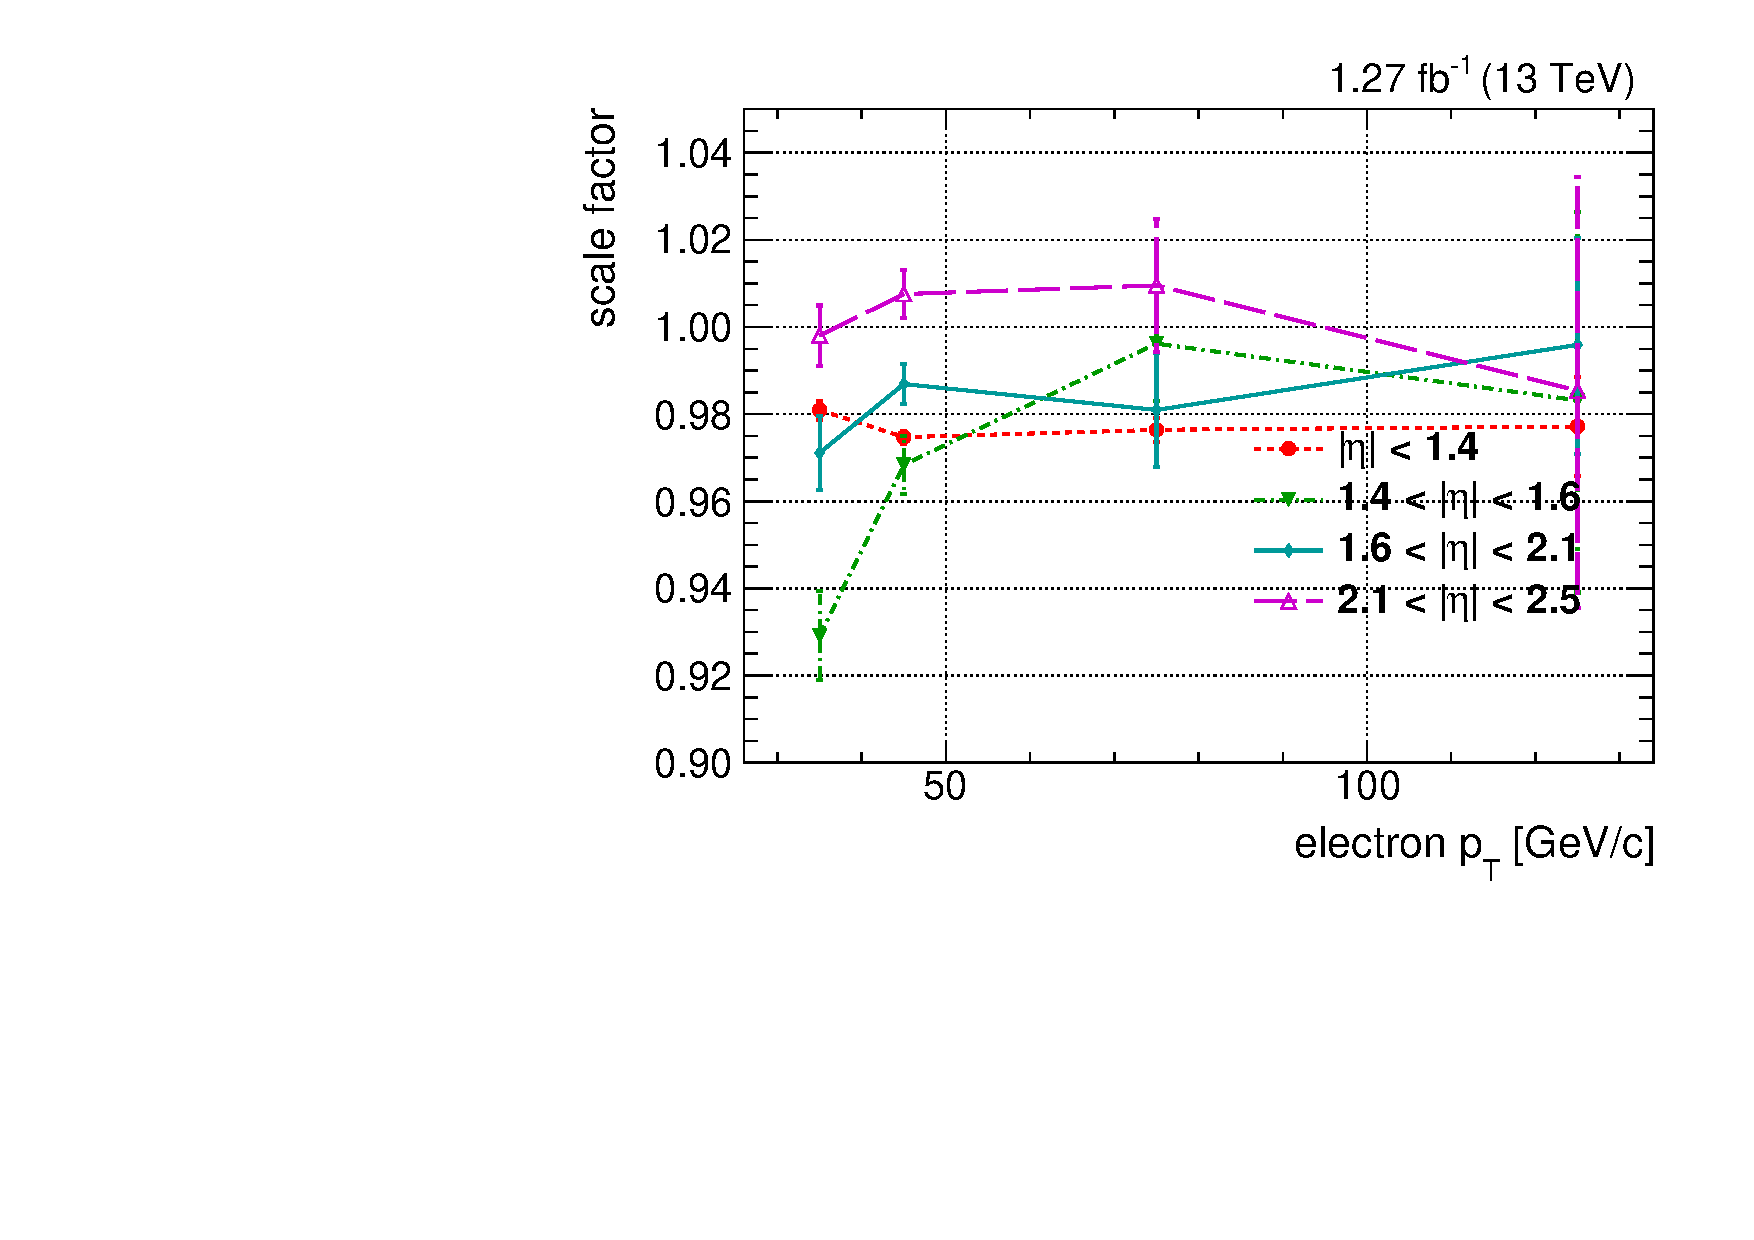
\includegraphics[width=0.48\textwidth]{figures/eletight_sfetapt.pdf}}
  \subfigure[]{\label{sub fig:eleloosesf}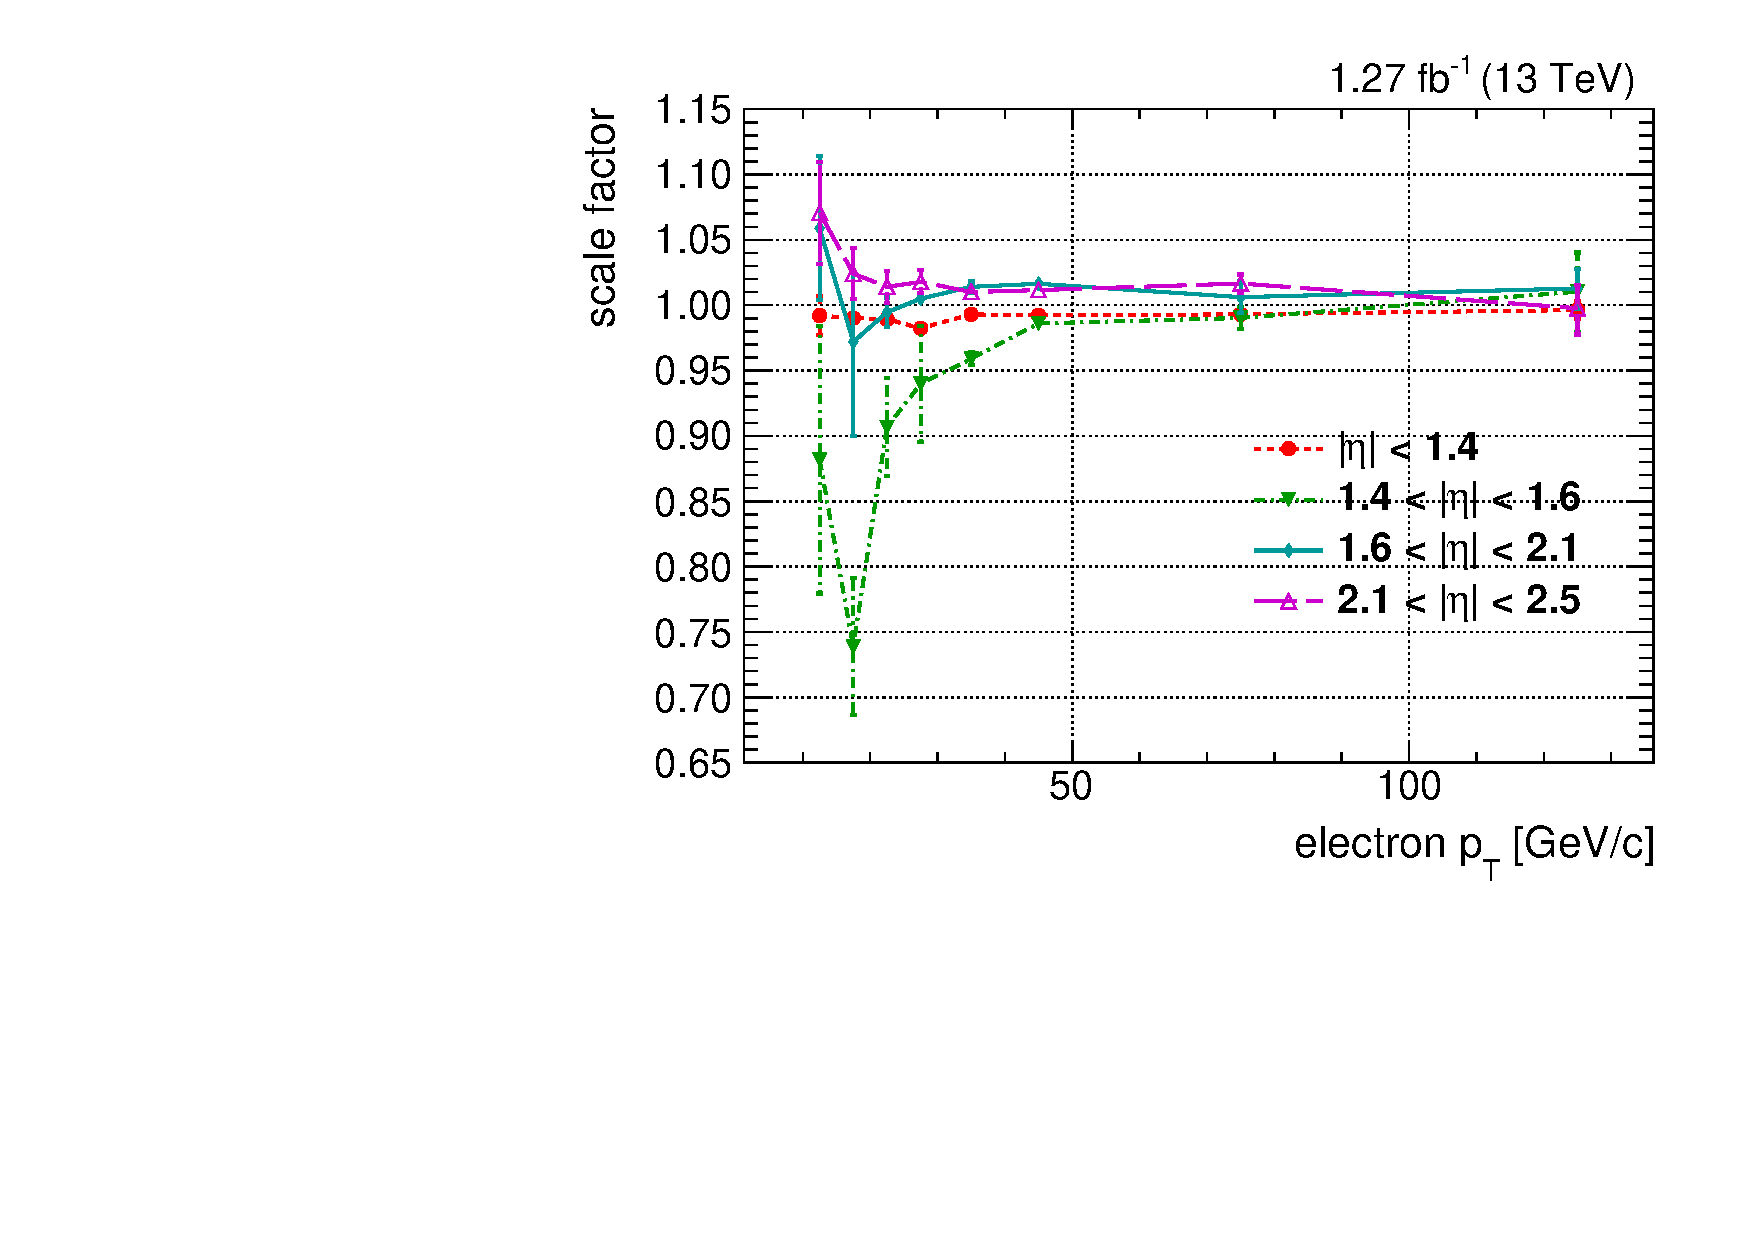
\includegraphics[width=0.48\textwidth]{figures/elveto_sfetapt.pdf}}
  \caption{Electron ``Tight" WP (left) and ``Veto" WP (right) data-to-MC efficiency scale factors as a function of electron $\pt$ for various $|\eta|$ bins.}
  \label{fig:ele_sf}	
\end{center}
\end{figure}

\begin{figure}[htbp]
\begin{center}
  \subfigure[]{\label{subfig:elvetoeffeta}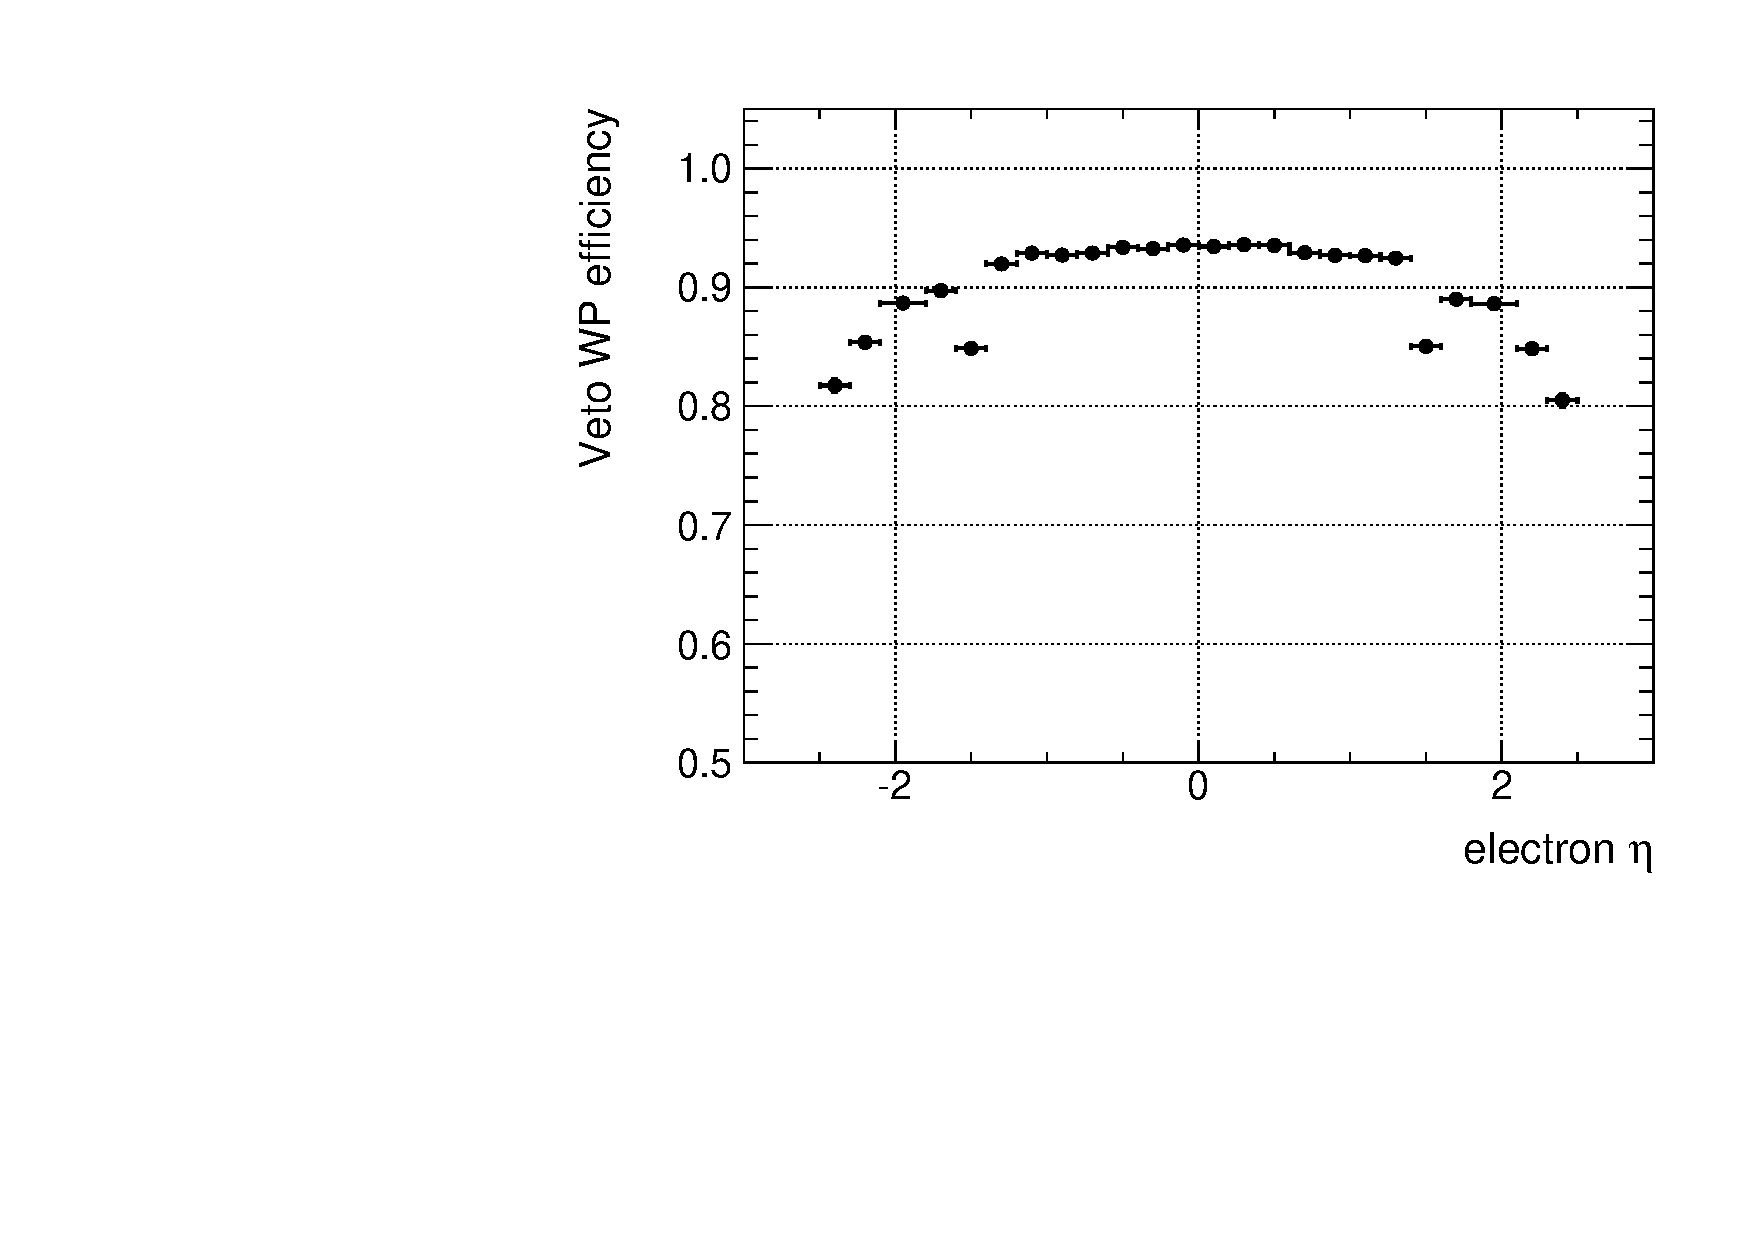
\includegraphics[width=0.48\textwidth]{figures/elveto_effeta.pdf}}
  \subfigure[]{\label{subfig:elvetoeffpt}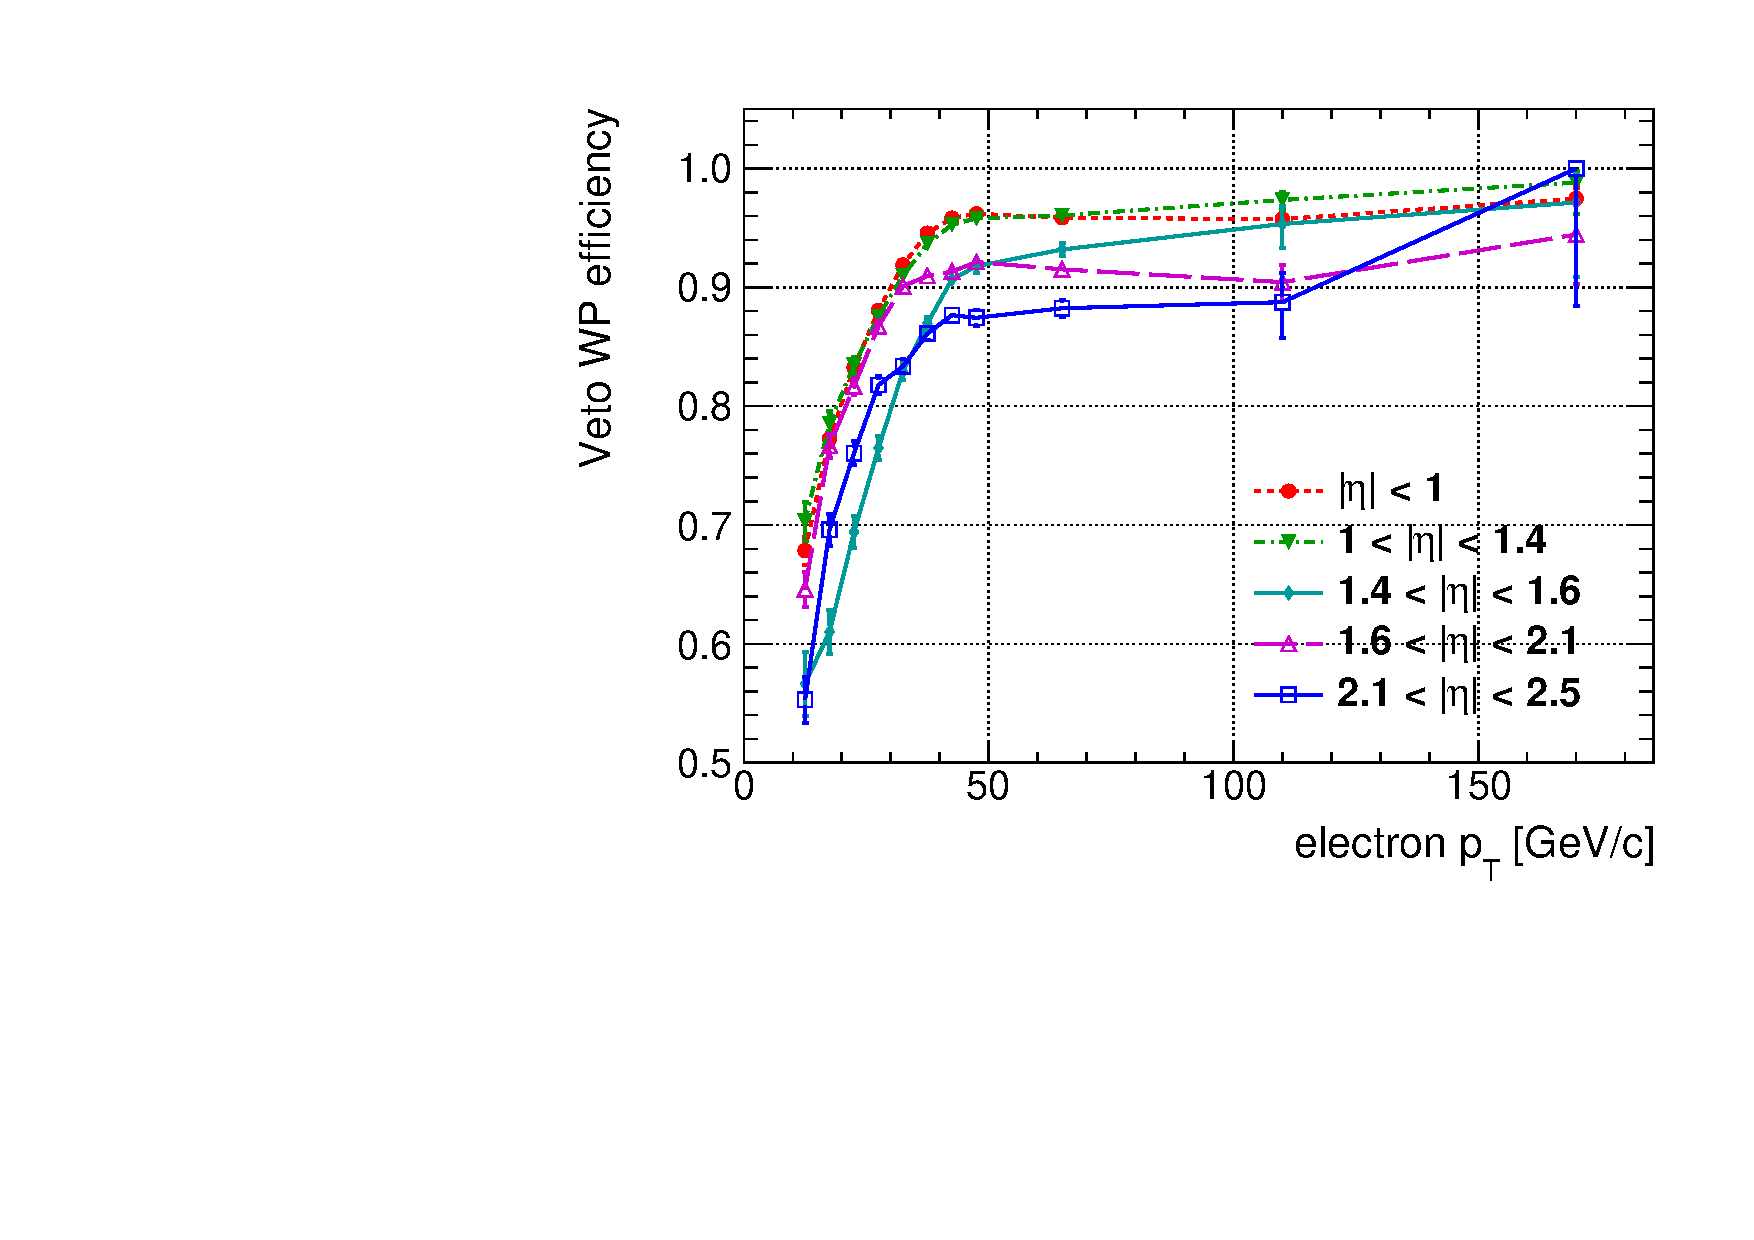
\includegraphics[width=0.48\textwidth]{figures/elveto_effetapt.pdf}}
  \caption{Electron ``Veto'' WP efficiencies with respect to \subref{subfig:elvetoeffeta} $\eta$ and \subref{subfig:elvetoeffpt} $\pt$ in different $|\eta|$-regions.}\textcolor{red}{Plots to be updated}
  \label{fig:elvetoeff}
\end{center}
\end{figure}

\begin{figure}[htbp]
\begin{center}
  \subfigure[]{\label{subfig:eltighteffeta}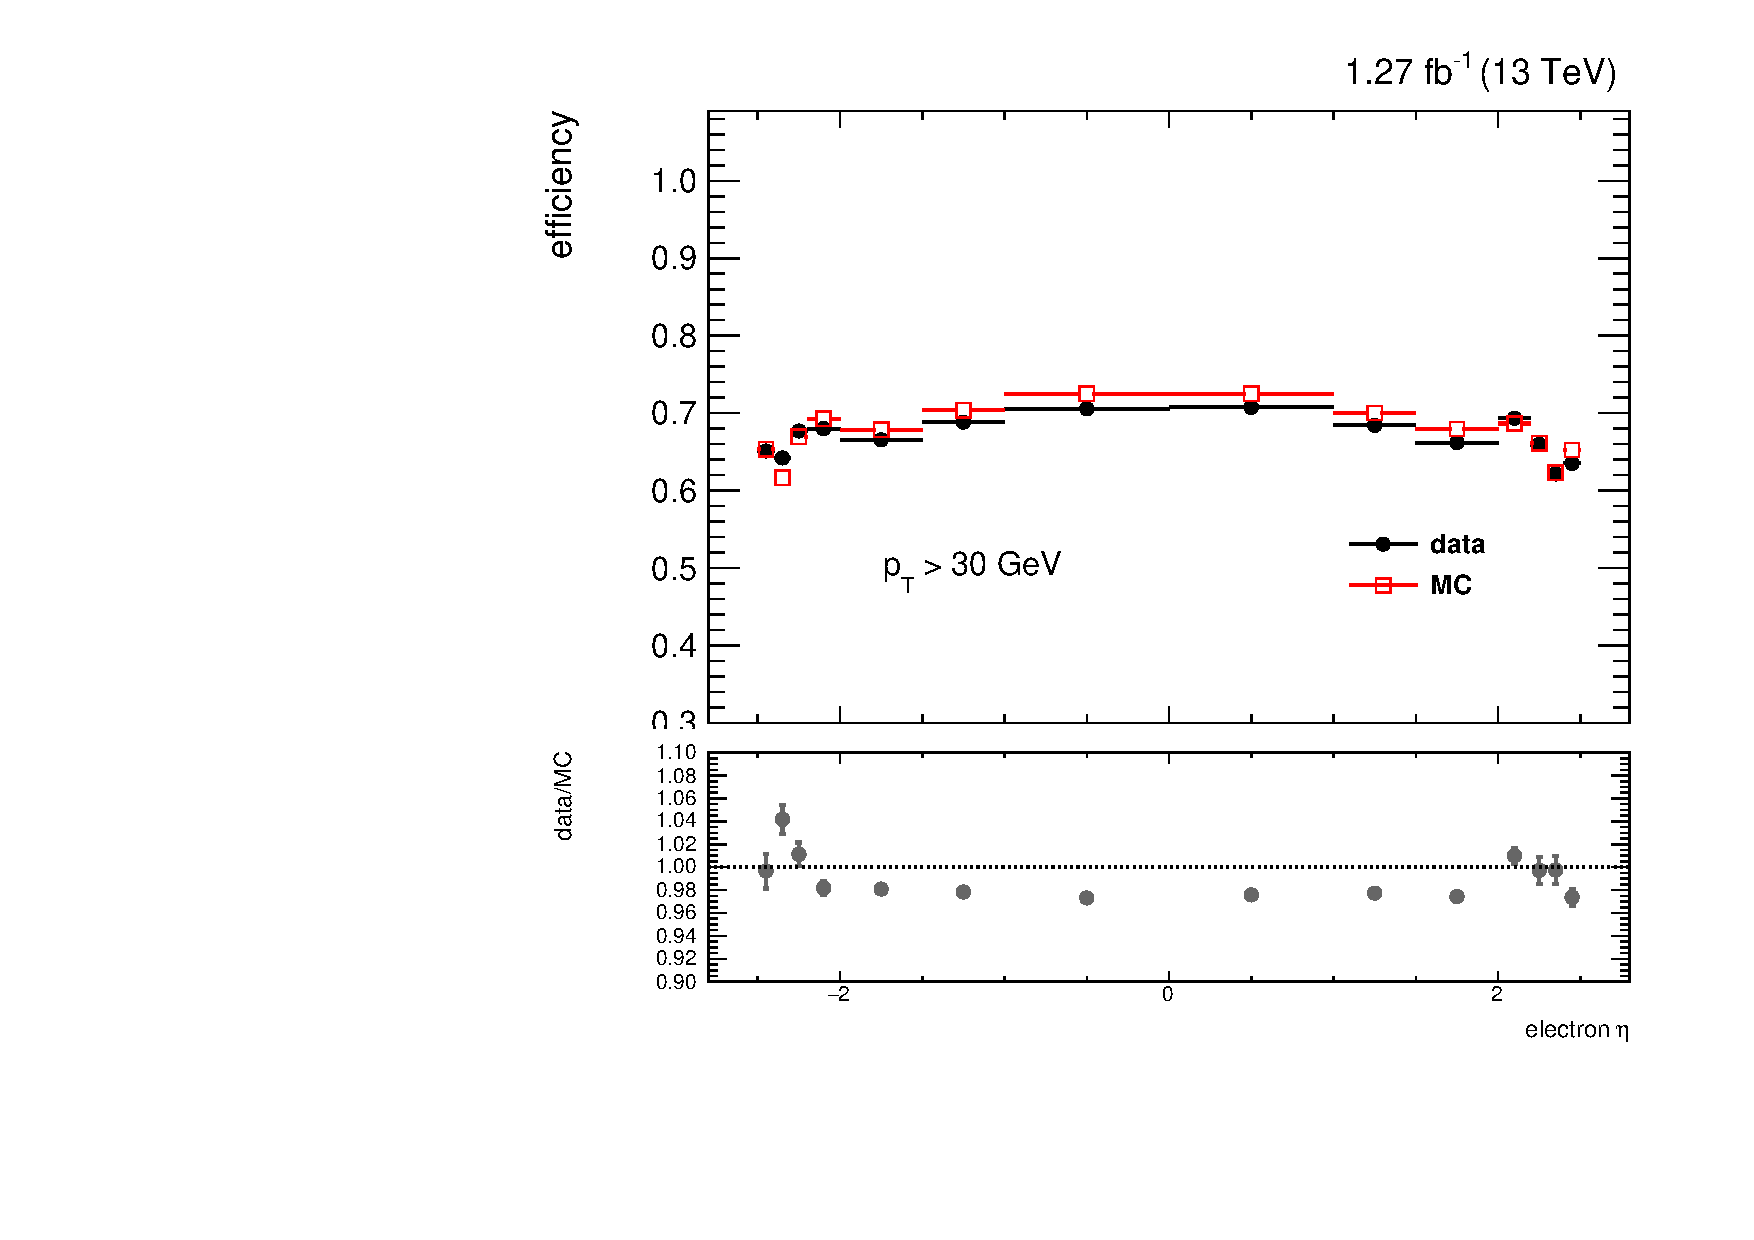
\includegraphics[width=0.48\textwidth]{figures/eltight_effeta_dataMC.pdf}}
  \subfigure[]{\label{subfig:eltighteffnpv}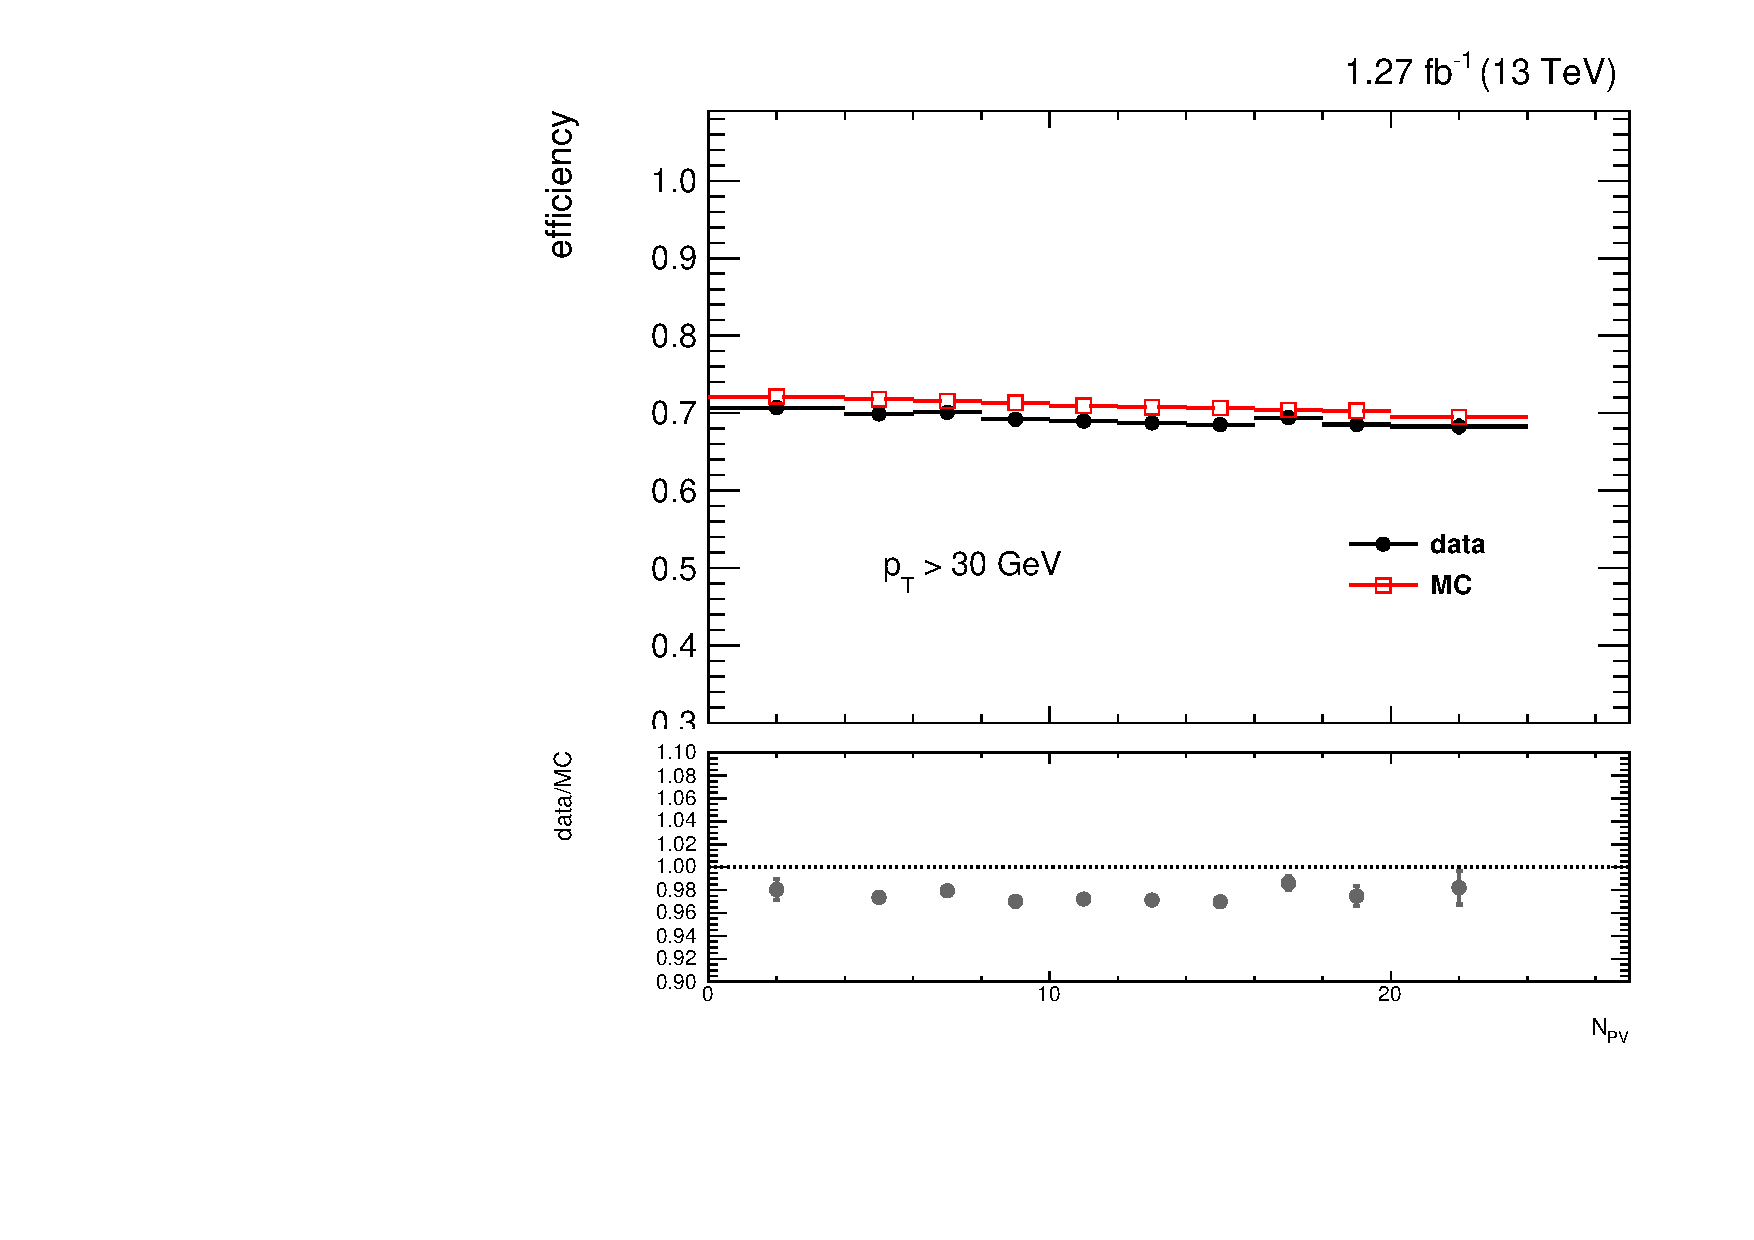
\includegraphics[width=0.48\textwidth]{figures/eltight_effnpv_dataMC.pdf}}
  \caption{Electron ``Tight'' WP efficiencies with respect to \subref{subfig:eltighteffeta} $\eta$ and \subref{subfig:eltighteffnpv} $N_{PV}$.}
  \label{fig:eltighteff}
\end{center}
\end{figure}
